\documentclass[
  shownotes,
  xcolor={svgnames},
  hyperref={colorlinks,citecolor=DarkBlue,linkcolor=andesred,urlcolor=DarkBlue}
  , aspectratio=169]{beamer}
\usepackage{animate}
\usepackage{amsmath}
\usepackage{amsfonts}
\usepackage{amssymb}
\usepackage{pifont}
\usepackage{mathpazo}
%\usepackage{xcolor}
\usepackage{multimedia}
\usepackage{fancybox}
\usepackage[para]{threeparttable}
\usepackage{multirow}
\setcounter{MaxMatrixCols}{30}
\usepackage{subcaption}
\usepackage{graphicx}
\usepackage{lscape}
\usepackage[compatibility=false,font=small]{caption}
\usepackage{booktabs}
\usepackage{ragged2e}
\usepackage{chronosys}
\usepackage{appendixnumberbeamer}
\usepackage{animate}
\setbeamertemplate{caption}[numbered]
\usepackage{color}
%\usepackage{times}
\usepackage{tikz}
\usepackage{comment} %to comment
%% BibTeX settings
\usepackage{natbib}
\bibliographystyle{apalike}
\bibpunct{(}{)}{,}{a}{,}{,}
\setbeamertemplate{bibliography item}{[\theenumiv]}

% Defines columns for bespoke tables
\usepackage{array}
\newcolumntype{L}[1]{>{\raggedright\let\newline\\\arraybackslash\hspace{0pt}}m{#1}}
\newcolumntype{C}[1]{>{\centering\let\newline\\\arraybackslash\hspace{0pt}}m{#1}}
\newcolumntype{R}[1]{>{\raggedleft\let\newline\\\arraybackslash\hspace{0pt}}m{#1}}


\usepackage{xfrac}


\usepackage{multicol}
\setlength{\columnsep}{0.5cm}

% Theme and colors
\usetheme{Boadilla}

% I define a custom pallete
\definecolor{andesred}{HTML}{1B175E}
\definecolor{andesyellow}{HTML}{ffff00}

% Other options
\providecommand{\U}[1]{\protect\rule{.1in}{.1in}}
\usefonttheme{serif}
\setbeamertemplate{itemize items}[default]
\setbeamertemplate{enumerate items}[square]
\setbeamertemplate{section in toc}[circle]


\definecolor{mybackground}{HTML}{1B175E}
\definecolor{myforeground}{HTML}{0000A0}

\setbeamercolor{normal text}{fg=black,bg=white}
\setbeamercolor{alerted text}{fg=andesred}
\setbeamercolor{example text}{fg=black}

\setbeamercolor{background canvas}{fg=myforeground, bg=white}
\setbeamercolor{background}{fg=myforeground, bg=mybackground}
\setbeamercolor{palette tertiary}{fg=myforeground,bg=mybackground}

\setbeamercolor{palette primary}{fg=black, bg=white}
\setbeamercolor{palette secondary}{fg=black, bg=white!10!andesyellow}
\setbeamercolor{palette tertiary}{fg=black, bg=white}


\setbeamercolor{frametitle}{fg=black}
\setbeamercolor{title}{fg=black}
\setbeamercolor{block title}{fg=andesred}
\setbeamercolor{itemize item}{fg=andesred}
\setbeamercolor{itemize subitem}{fg=andesred}
\setbeamercolor{itemize subsubitem}{fg=andesred}
\setbeamercolor{enumerate item}{fg=andesred}
\setbeamercolor{item projected}{bg=gray!30!white,fg=andesred}
\setbeamercolor{enumerate subitem}{fg=andesred}
\setbeamercolor{section number projected}{bg=gray!30!white,fg=andesred}
\setbeamercolor{section in toc}{fg=andesred}
\setbeamercolor{caption name}{fg=andesred}
\setbeamercolor{button}{bg=gray!30!white,fg=andesred}
\setbeamercolor{title in head/foot}{fg=andesred}



\usepackage{fancyvrb}
\newcommand{\VerbBar}{|}
\newcommand{\VERB}{\Verb[commandchars=\\\{\}]}
\DefineVerbatimEnvironment{Highlighting}{Verbatim}{commandchars=\\\{\}}
% Add ',fontsize=\small' for more characters per line
\usepackage{framed}
\definecolor{shadecolor}{RGB}{248,248,248}
\newenvironment{Shaded}{\begin{snugshade}}{\end{snugshade}}
\newcommand{\AlertTok}[1]{\textcolor[rgb]{0.94,0.16,0.16}{#1}}
\newcommand{\AnnotationTok}[1]{\textcolor[rgb]{0.56,0.35,0.01}{\textbf{\textit{#1}}}}
\newcommand{\AttributeTok}[1]{\textcolor[rgb]{0.77,0.63,0.00}{#1}}
\newcommand{\BaseNTok}[1]{\textcolor[rgb]{0.00,0.00,0.81}{#1}}
\newcommand{\BuiltInTok}[1]{#1}
\newcommand{\CharTok}[1]{\textcolor[rgb]{0.31,0.60,0.02}{#1}}
\newcommand{\CommentTok}[1]{\textcolor[rgb]{0.56,0.35,0.01}{\textit{#1}}}
\newcommand{\CommentVarTok}[1]{\textcolor[rgb]{0.56,0.35,0.01}{\textbf{\textit{#1}}}}
\newcommand{\ConstantTok}[1]{\textcolor[rgb]{0.00,0.00,0.00}{#1}}
\newcommand{\ControlFlowTok}[1]{\textcolor[rgb]{0.13,0.29,0.53}{\textbf{#1}}}
\newcommand{\DataTypeTok}[1]{\textcolor[rgb]{0.13,0.29,0.53}{#1}}
\newcommand{\DecValTok}[1]{\textcolor[rgb]{0.00,0.00,0.81}{#1}}
\newcommand{\DocumentationTok}[1]{\textcolor[rgb]{0.56,0.35,0.01}{\textbf{\textit{#1}}}}
\newcommand{\ErrorTok}[1]{\textcolor[rgb]{0.64,0.00,0.00}{\textbf{#1}}}
\newcommand{\ExtensionTok}[1]{#1}
\newcommand{\FloatTok}[1]{\textcolor[rgb]{0.00,0.00,0.81}{#1}}
\newcommand{\FunctionTok}[1]{\textcolor[rgb]{0.00,0.00,0.00}{#1}}
\newcommand{\ImportTok}[1]{#1}
\newcommand{\InformationTok}[1]{\textcolor[rgb]{0.56,0.35,0.01}{\textbf{\textit{#1}}}}
\newcommand{\KeywordTok}[1]{\textcolor[rgb]{0.13,0.29,0.53}{\textbf{#1}}}
\newcommand{\NormalTok}[1]{#1}
\newcommand{\OperatorTok}[1]{\textcolor[rgb]{0.81,0.36,0.00}{\textbf{#1}}}
\newcommand{\OtherTok}[1]{\textcolor[rgb]{0.56,0.35,0.01}{#1}}
\newcommand{\PreprocessorTok}[1]{\textcolor[rgb]{0.56,0.35,0.01}{\textit{#1}}}
\newcommand{\RegionMarkerTok}[1]{#1}
\newcommand{\SpecialCharTok}[1]{\textcolor[rgb]{0.00,0.00,0.00}{#1}}
\newcommand{\SpecialStringTok}[1]{\textcolor[rgb]{0.31,0.60,0.02}{#1}}
\newcommand{\StringTok}[1]{\textcolor[rgb]{0.31,0.60,0.02}{#1}}
\newcommand{\VariableTok}[1]{\textcolor[rgb]{0.00,0.00,0.00}{#1}}
\newcommand{\VerbatimStringTok}[1]{\textcolor[rgb]{0.31,0.60,0.02}{#1}}
\newcommand{\WarningTok}[1]{\textcolor[rgb]{0.56,0.35,0.01}{\textbf{\textit{#1}}}}
\usepackage{graphicx}
\makeatletter

\makeatother






%%%%%%%%%%%%%%% BEGINS DOCUMENT %%%%%%%%%%%%%%%%%%

\AtBeginSection[]
{
    \begin{frame}
        \frametitle{Agenda}
        \tableofcontents[currentsection]
    \end{frame}
}



\AtBeginSubsection[]
{
    \begin{frame}
        \frametitle{Agenda}
        \tableofcontents[currentsubsection]
    \end{frame}
}

\begin{document}

\title{Selección de Modelos y Regularización}
\subtitle{Big Data y Machine Learning para Economía Aplicada}
\date{}

\author[Sarmiento-Barbieri]{Ignacio Sarmiento-Barbieri}
\institute[Uniandes]{Universidad de los Andes}



%----------------------------------------------------------------------%
\begin{frame}[noframenumbering]
\maketitle
\end{frame}
%----------------------------------------------------------------------%
\begin{frame}
\frametitle{Agenda}

\tableofcontents


\end{frame}
%----------------------------------------------------------------------%
\section{Recap: Predicción y Overfit} 
%----------------------------------------------------------------------%

%----------------------------------------------------------------------%
\begin{frame}[fragile, noframenumbering]
\frametitle{Overfit y Predicción fuera de Muestra}


        \begin{figure}[H] \centering
            \captionsetup{justification=centering}
              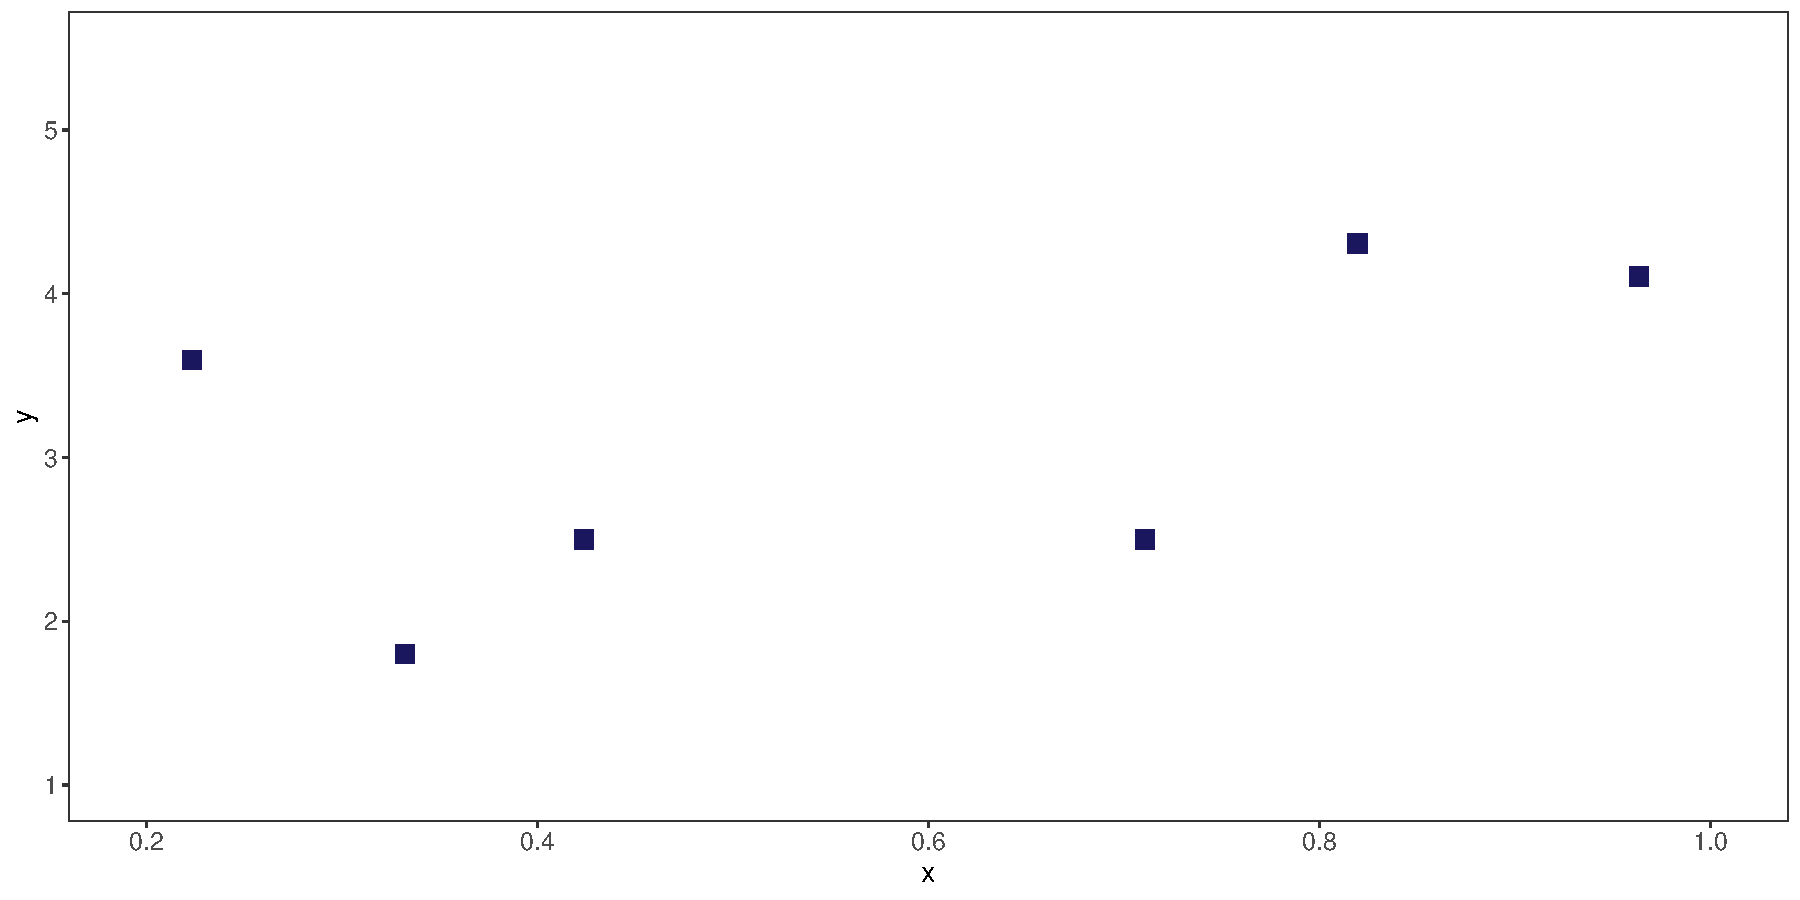
\includegraphics[scale=0.4]{figures/fig_1a.pdf}
 \end{figure}


\end{frame}

%----------------------------------------------------------------------%
\begin{frame}[fragile, noframenumbering]
\frametitle{Overfit y Predicción fuera de Muestra}


        \begin{figure}[H] \centering
            \captionsetup{justification=centering}
              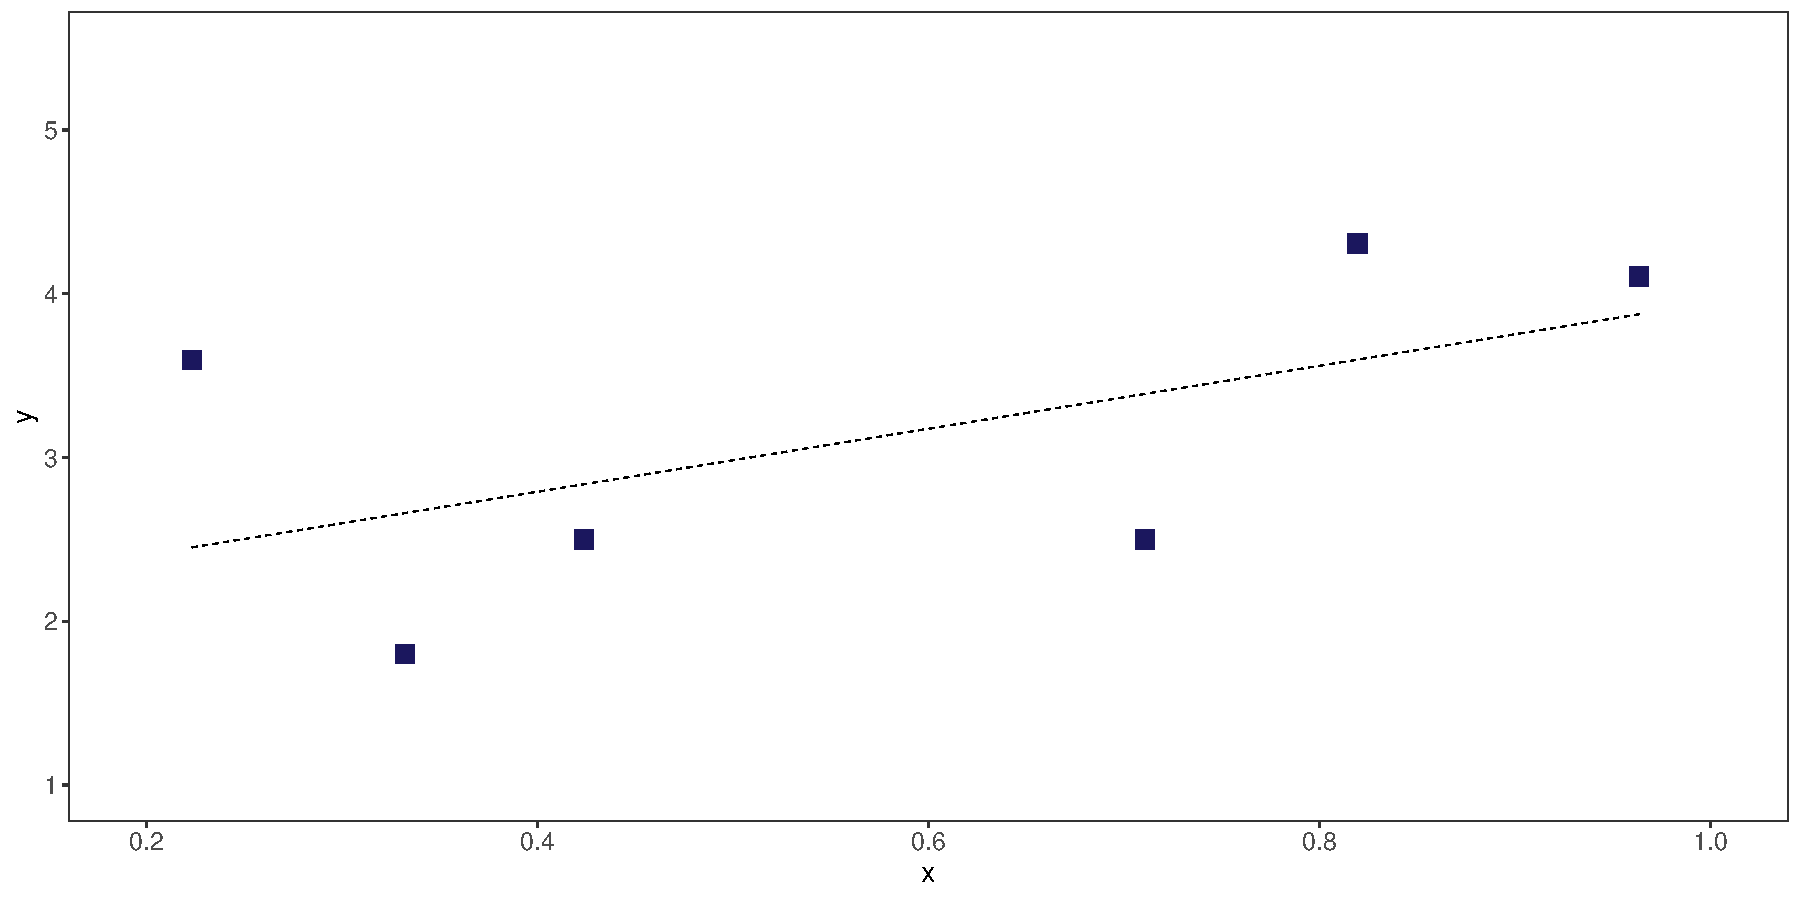
\includegraphics[scale=0.4]{figures/fig_1_poly1.pdf}
 \end{figure}



\end{frame}

%----------------------------------------------------------------------%
\begin{frame}[fragile, noframenumbering]
\frametitle{Overfit y Predicción fuera de Muestra}


        \begin{figure}[H] \centering
            \captionsetup{justification=centering}
              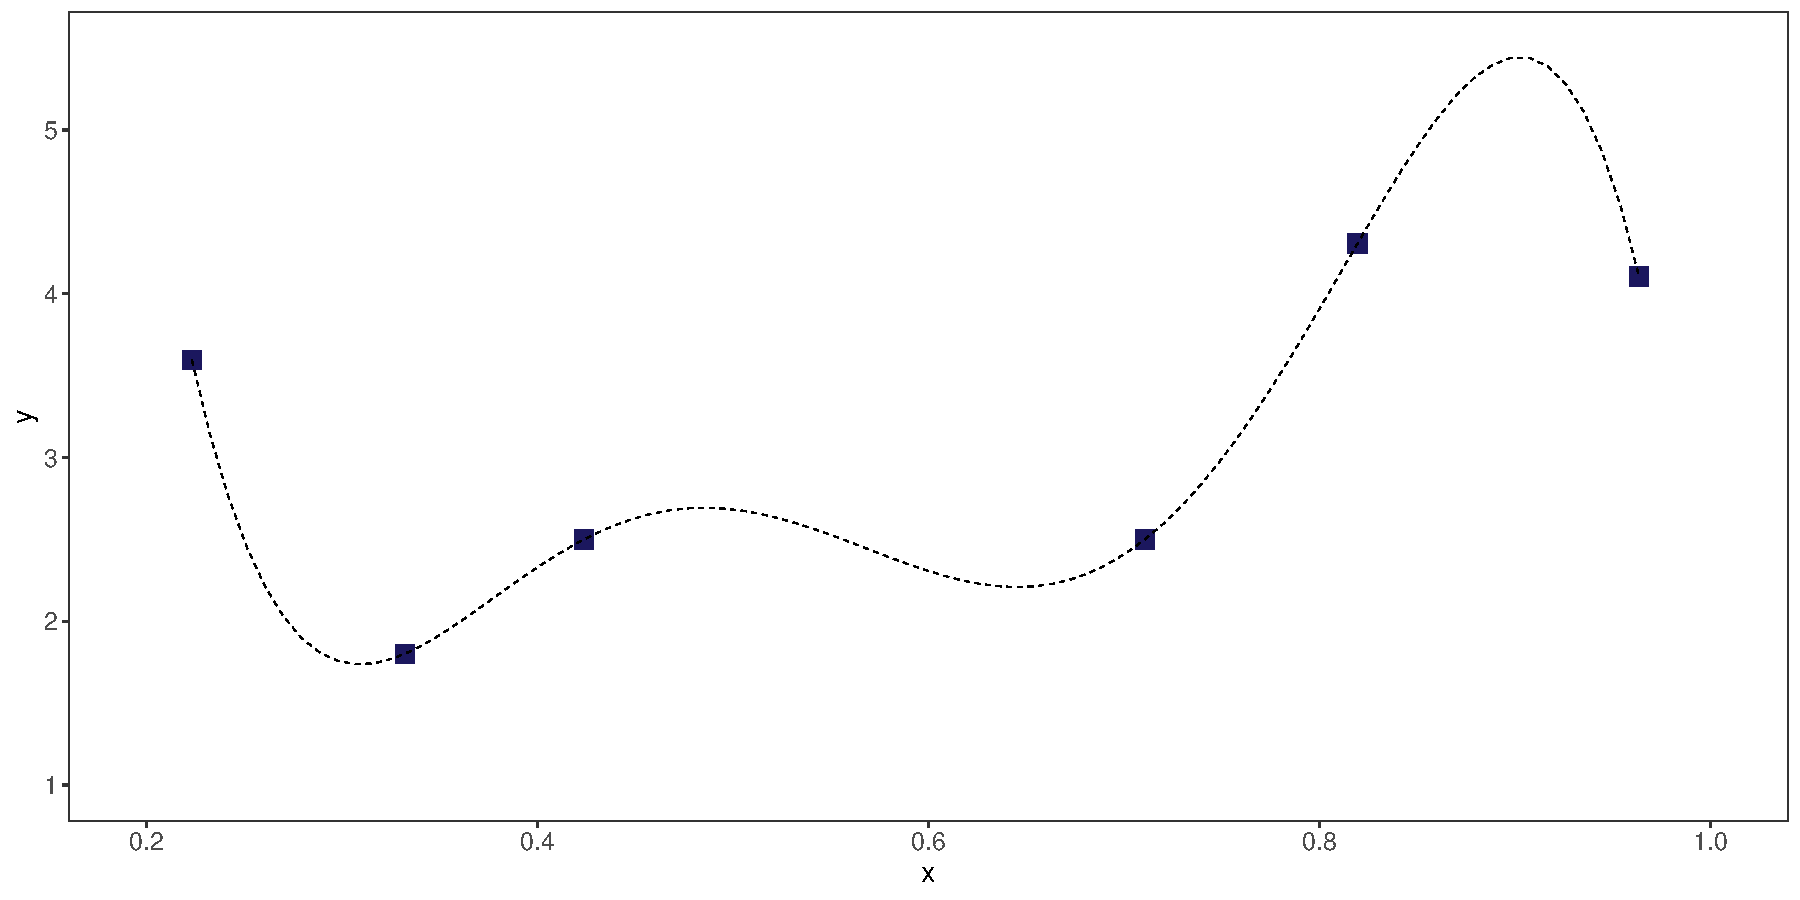
\includegraphics[scale=0.4]{figures/fig_1_poly5.pdf}
 \end{figure}

\end{frame}

%----------------------------------------------------------------------%
\begin{frame}[fragile, noframenumbering]
\frametitle{Overfit y Predicción fuera de Muestra}


        \begin{figure}[H] \centering
            \captionsetup{justification=centering}
              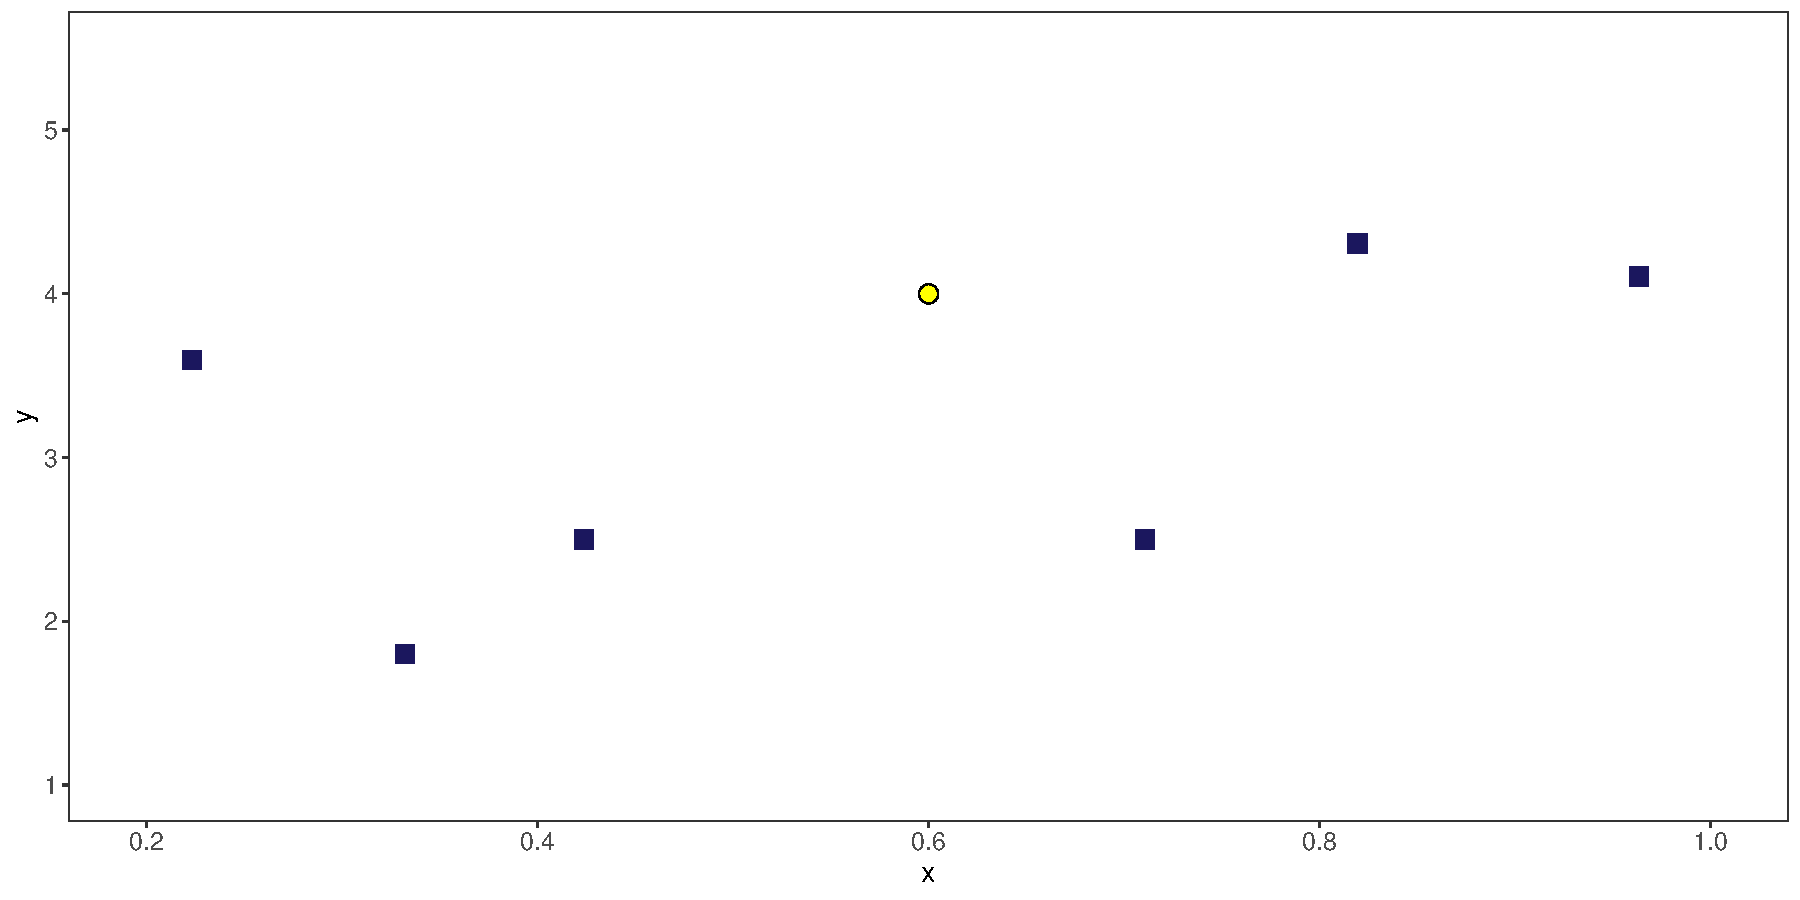
\includegraphics[scale=0.4]{figures/fig_all_sample.pdf}
 \end{figure}

\end{frame}

%----------------------------------------------------------------------%
\begin{frame}[fragile, noframenumbering]
\frametitle{Overfit y Predicción fuera de Muestra}


        \begin{figure}[H] \centering
            \captionsetup{justification=centering}
              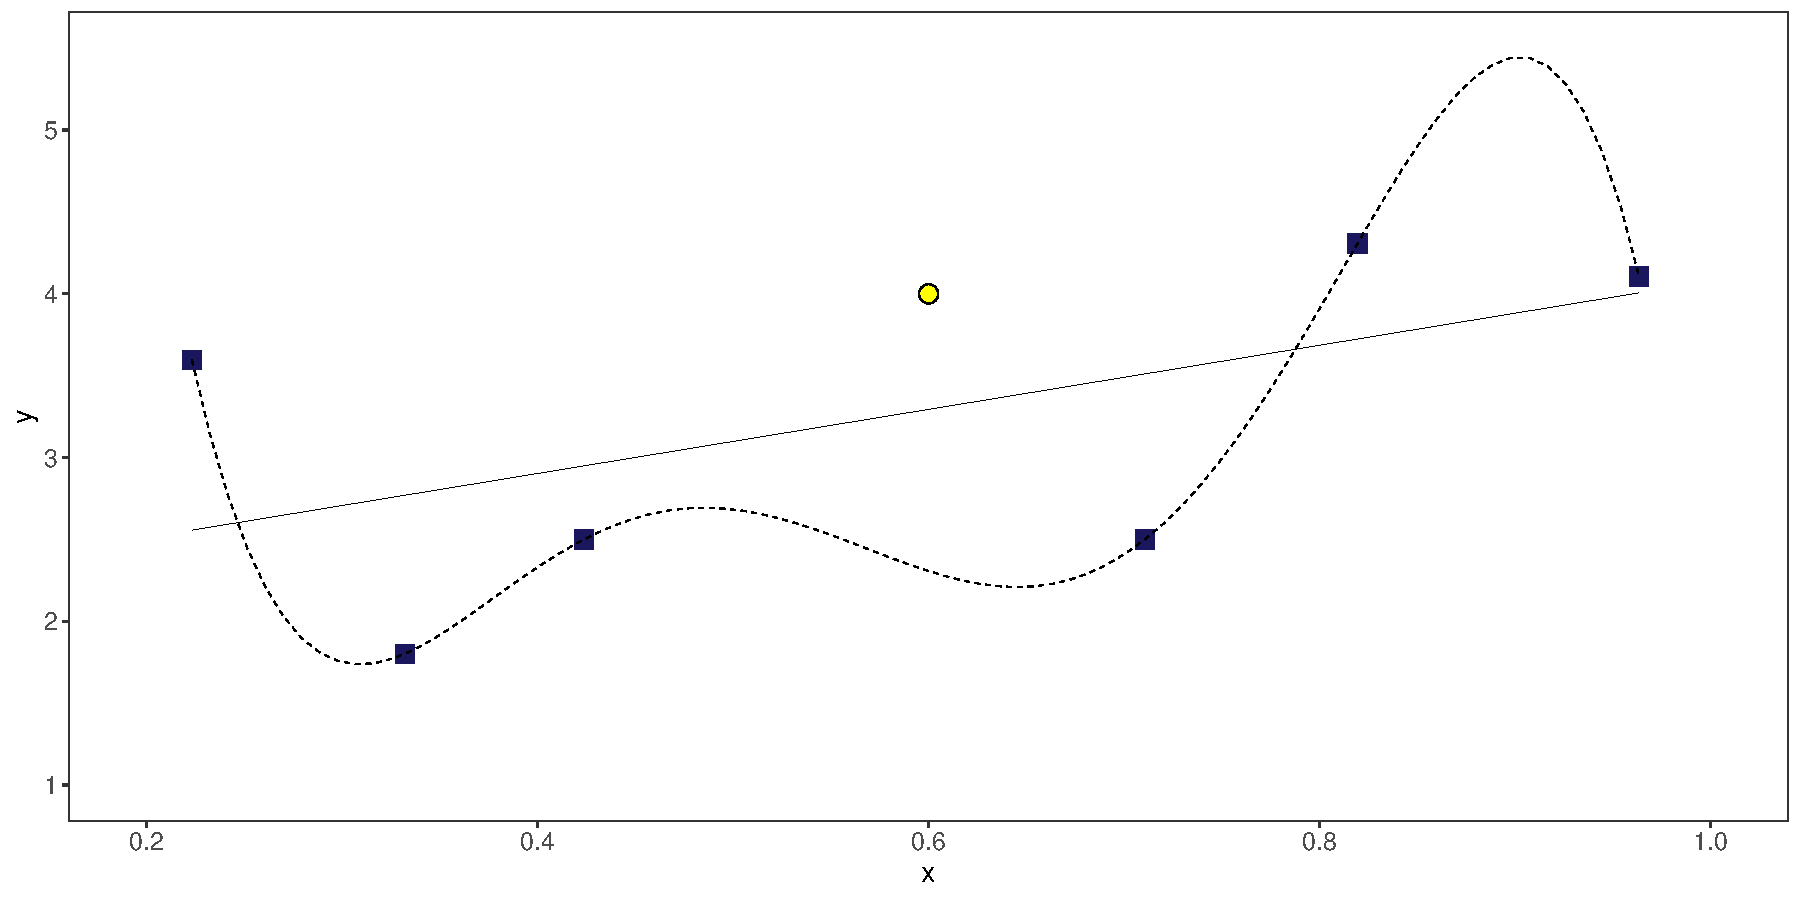
\includegraphics[scale=0.4]{figures/fig_all_sample_polys.pdf}
 \end{figure}


\end{frame}

%----------------------------------------------------------------------%
\begin{frame}[fragile, noframenumbering]
\frametitle{Overfit y Predicción fuera de Muestra}


        \begin{figure}[H] \centering
            \captionsetup{justification=centering}
              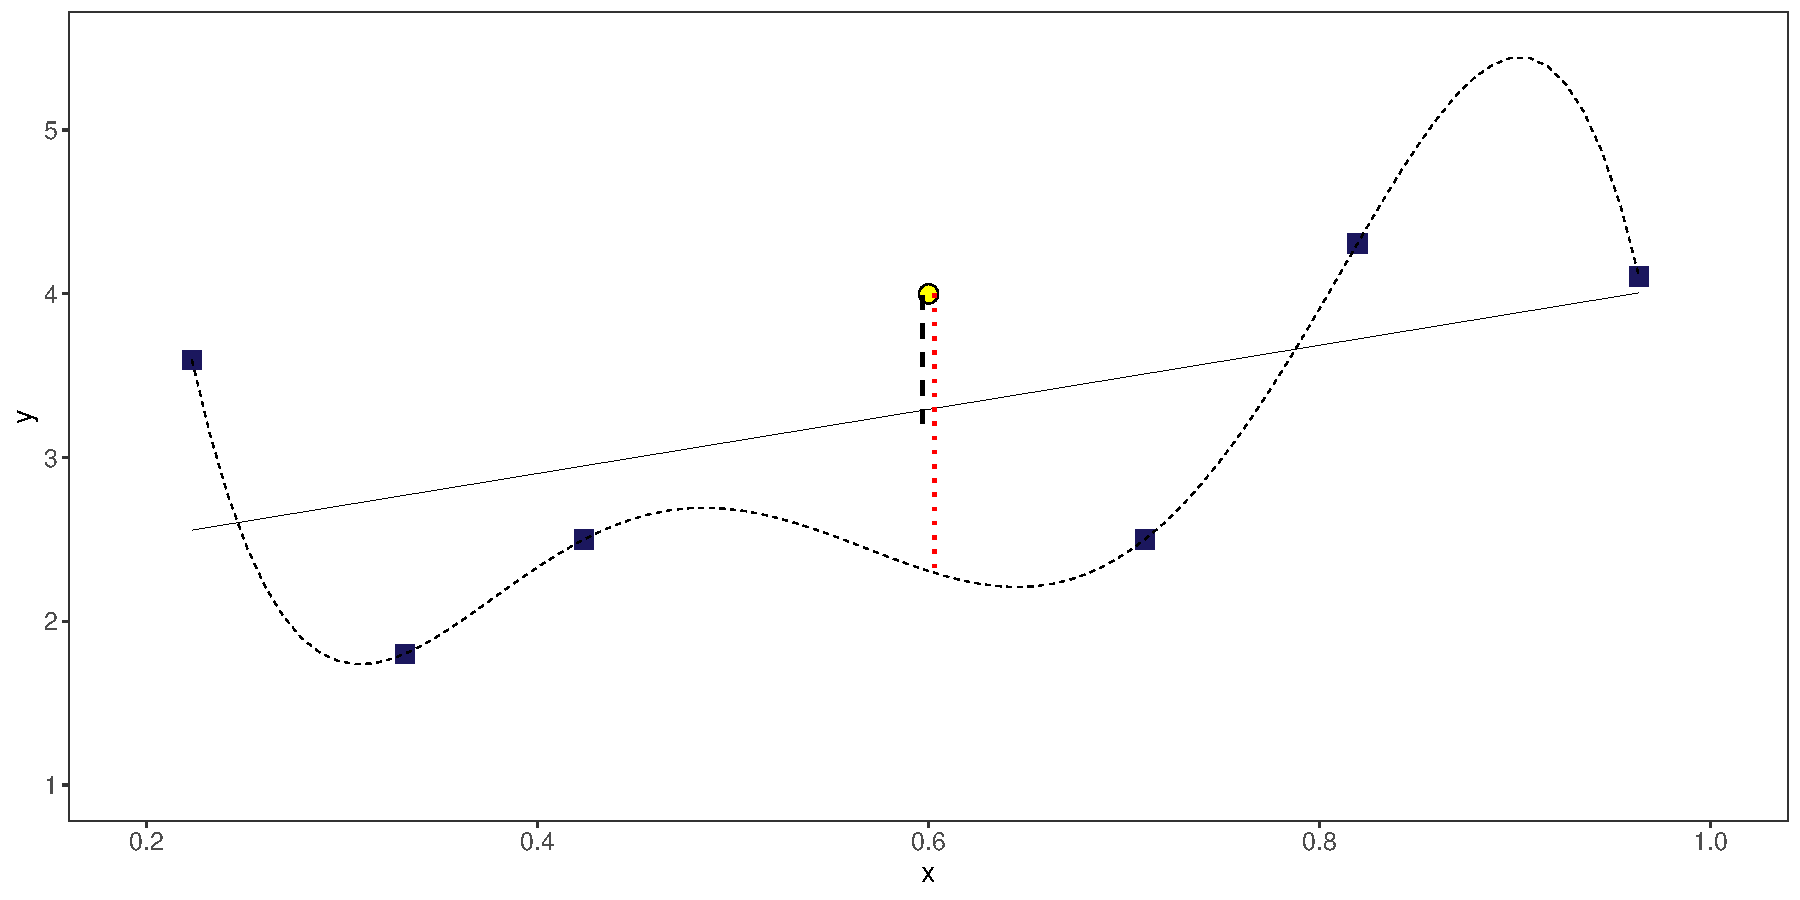
\includegraphics[scale=0.4]{figures/fig_all_sample_polys_erors_all.pdf}
 \end{figure}


\end{frame}
%----------------------------------------------------------------------%
\begin{frame}
\frametitle{Overfit y Predicción fuera de Muestra}



\begin{figure}[H] \centering
            \captionsetup{justification=centering}  
            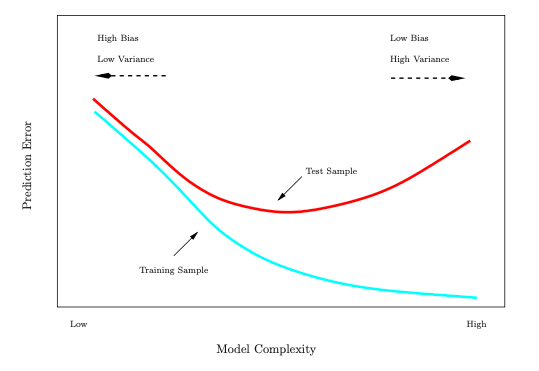
\includegraphics[scale=.6]{figures/train_test_error.png}
    \end{figure}

\end{frame}
%----------------------------------------------------------------------%
\begin{frame}
\frametitle{Overfit y Predicción fuera de Muestra}


\begin{itemize}
  \item ML nos interesa la predicción fuera de muestra
  \medskip
  \item Overfit: modelos complejos predicen muy bien dentro de muestra, pero tienden a hacer un mal trabajo fuera de muestra 
  \medskip
  \item Hay que elegir el modelo que ``mejor'' prediga fuera de muestra (out-of-sample)
  \medskip

    \begin{itemize}
    \medskip
    \item Métodos de Remuestreo
    \medskip
      \begin{itemize}

        \item Enfoque del conjunto de validación
        \medskip
        \item LOOCV
        \medskip
        \item Validación cruzada en K-partes (5 o 10)
      \end{itemize}
    \end{itemize}

\end{itemize}

\end{frame}
%----------------------------------------------------------------------%
\begin{frame}[fragile]
\frametitle{}
\begin{figure}[H] \centering
  \centering
  
\includegraphics[scale=0.35]{figures/baticomputer_meme.jpg}
  \\
  \tiny photo from \url{https://www.dailydot.com/parsec/batman-1966-labels-tumblr-twitter-vine/}
\end{figure}

 \end{frame}
%----------------------------------------------------------------------%
%----------------------------------------------------------------------%
\section{Regularización}
%----------------------------------------------------------------------%
\begin{frame}<1>[label=motivacion]
\frametitle{Regularización: Motivación}

\begin{itemize}
\item Las técnicas econometricas estándar no están optimizadas para la predicción porque se enfocan en la insesgadez.
\medskip
\item OLS por ejemplo es el mejor estimador lineal {\it insesgado}
\medskip
\item OLS minimiza el error {\it ``dentro de muestra''}, eligiendo $\beta$ de forma tal que 


\begin{align}
min_{\beta} E(\beta) = \sum_{i=1}^n (y_i-\beta_0 - x_{i1}\beta_1 - \dots - x_{ip}\beta_p)^2 
\end{align}

\pause
\item pero para predicción, no estamos interesados en hacer un buen trabajo dentro de muestra 
\medskip
\item Queremos hacer un buen trabajo, {\bf fuera de muestra}
\end{itemize}
\end{frame}
%----------------------------------------------------------------------%
\subsection{Recap: OLS Mechanics}
%----------------------------------------------------------------------%
%----------------------------------------------------------------------%
\begin{frame}[fragile]
\frametitle{OLS 1 Dimension}
\footnotesize
\begin{align}
 min_{\beta} E(\beta)=\sum_{i=1}^n (y_i-x_i \beta)^2 
\end{align}
   \begin{figure}[H] \centering
            \captionsetup{justification=centering}
              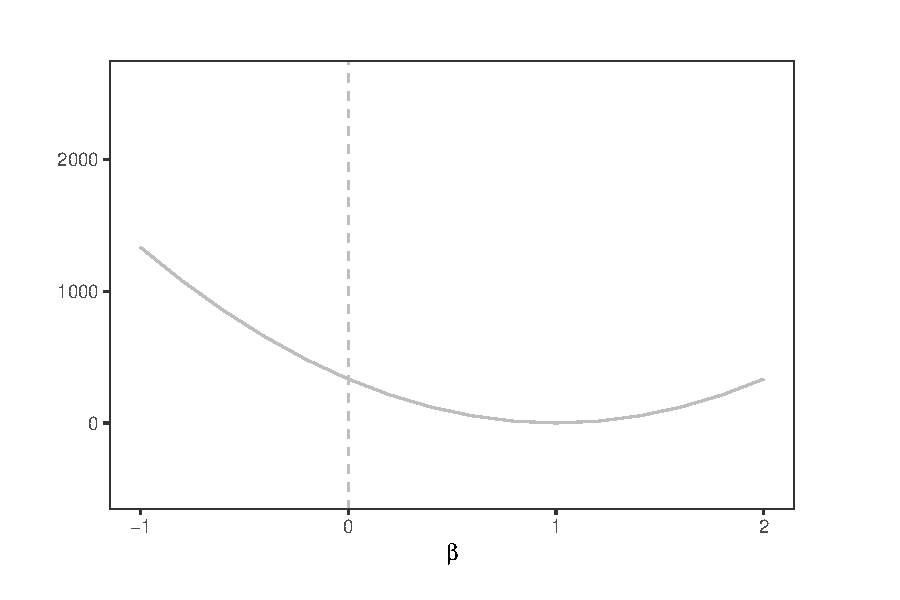
\includegraphics[scale=0.4]{figures/lasso0.pdf}
 \end{figure}

Solución

\begin{align}
\frac{\partial E(\beta)}{\partial \beta}= \sum_{i=1}^n 2(y_i-x_i \beta)(-x_i )
\end{align}

\href{https://cede.uniandes.edu.co/OLS/}{App}

\end{frame}
%----------------------------------------------------------------------%
\begin{frame}[fragile]
\frametitle{OLS 1 Dimension}
\begin{align}
\frac{\partial E(\beta)}{\partial \beta}= \sum_{i=1}^n 2(y_i-x_i \beta)(-x_i )
\end{align}

\begin{align}
\hat{\beta} = \frac{\sum y_ix_i}{\sum x^2_i}
\end{align}
\end{frame}
%----------------------------------------------------------------------%
\begin{frame}[fragile]
\frametitle{OLS 2 Dimensiones}
\footnotesize
\begin{align}
min_{\beta} E(\beta) = \sum_{i=1}^n (y_i - x_{i1}\beta_1-x_{i2}\beta_2)^2 
\end{align}
\begin{figure}[H] \centering
            \captionsetup{justification=centering}
              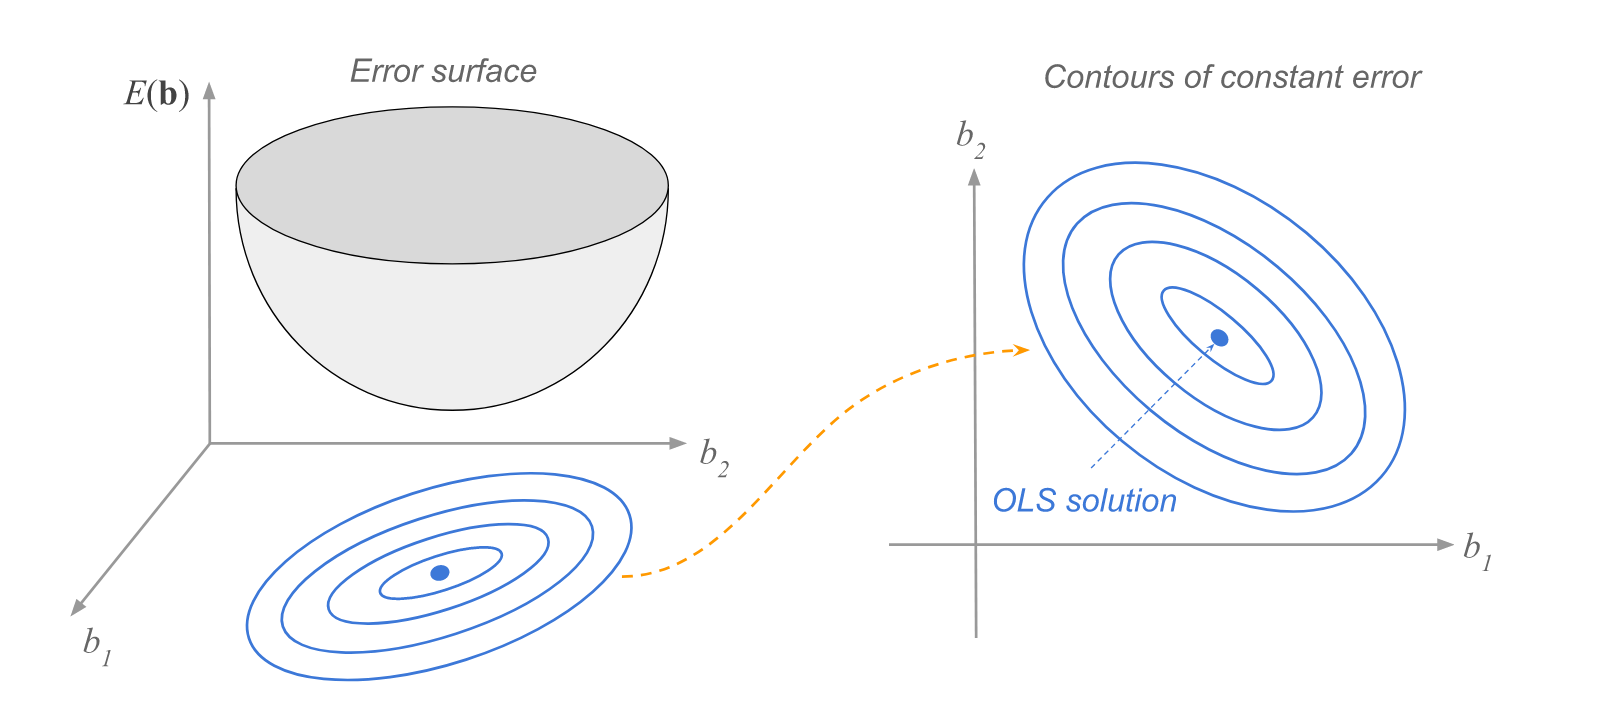
\includegraphics[scale=0.4]{figures/ols1}
 
\tiny
Fuente: \url{https://allmodelsarewrong.github.io}
\end{figure}

\href{https://cede.uniandes.edu.co/OLS/}{App}
\end{frame}

%----------------------------------------------------------------------%
%----------------------------------------------------------------------%
\againframe<2>{motivacion}
%----------------------------------------------------------------------%
%----------------------------------------------------------------------%
%----------------------------------------------------------------------%
\subsection{Ridge}
%----------------------------------------------------------------------%
\begin{frame}[fragile]
\frametitle{Ridge}
  \begin{itemize}
    \item Asegurar cero sesgo dentro de muestra crea problemas fuera de muestra: trade-off Sesgo-Varianza
    \medskip
    \item Las técnicas de machine learning fueron desarrolladas para hacer este trade-off de forma empírica.
    \medskip
    \item Vamos a proponer modelos del estilo


\begin{align}
min_{\beta} E(\beta) = \sum_{i=1}^n (y_i-\beta_0 - x_{i1}\beta_1 - \dots - x_{ip}\beta_p)^2 + \lambda \sum_{j=1}^p R(\beta_j)
\end{align}

\item donde $R$ es un regularizador que penaliza funciones que crean varianza
\medskip
\item Explícitamente en la minimización incluimos un termino de sesgo y un termino de varianza.


  \end{itemize}
\end{frame}
%----------------------------------------------------------------------%
\begin{frame}[fragile]
\frametitle{Ridge}

\begin{itemize}
\item Para un $\lambda \geq 0$ dado, consideremos ahora el siguiente problema de optimización


\begin{align}
min_{\beta} E(\beta) = \sum_{i=1}^n (y_i-\beta_0 - x_{i1}\beta_1 - \dots - x_{ip}\beta_p)^2 + \lambda \sum_{j=1}^p (\beta_j)^2
\end{align}



\end{itemize}
\end{frame}
%----------------------------------------------------------------------%
\begin{frame}[fragile]
\frametitle{Ridge: Intuición en 1 Dimension }

\begin{itemize}
\item 1 predictor estandarizado
\medskip
\item El problema entonces es 
\begin{align}
min_{\beta} E(\beta) = \sum_{i=1}^n (y_i- x_{i}\beta )^2 + \lambda \beta^2
\end{align}

\item La solución?

\vspace{2in}
\href{https://cede.uniandes.edu.co/OLS/}{App}
\end{itemize}
\end{frame}
%----------------------------------------------------------------------%
\begin{frame}[fragile]
\frametitle{Ridge: Intuición en 2 Dimensiones }

\begin{itemize}
\item Al problema en 2 dimensiones podemos escribirlo como

  \begin{align}
  min_{\beta} E(\beta) = \sum_{i=1}^n (y_i  - x_{i1}\beta_1  - x_{i2}\beta_2 + \lambda  \left(\beta_1^2 + \beta_2^2 \right)
  \end{align}
\medskip 
\item podemos escribirlo como un problema de optimización restringido
  \begin{align}
     min_{\beta} E(\beta) &= \sum_{i=1}^n (y_i - x_{i1}\beta_1 - x_{i1}\beta_2)^2  \\ \nonumber
     & \text{sujeto a}   \\
     & \left( (\beta_1)^2 + (\beta_2)^2 \right) \leq c \nonumber
  \end{align}

\end{itemize}

\end{frame}
%----------------------------------------------------------------------%
\begin{frame}[fragile]
\frametitle{Ridge: Intuición en 2 Dimensiones }

\begin{align}
     min_{\beta} E(\beta) &= \sum_{i=1}^n (y_i - x_{i1}\beta_1 - x_{i1}\beta_2)^2  \text{ s.a }   \left( (\beta_1)^2 + (\beta_2)^2 \right) \leq c 
  \end{align}

\begin{figure}[H] \centering
            \captionsetup{justification=centering}
              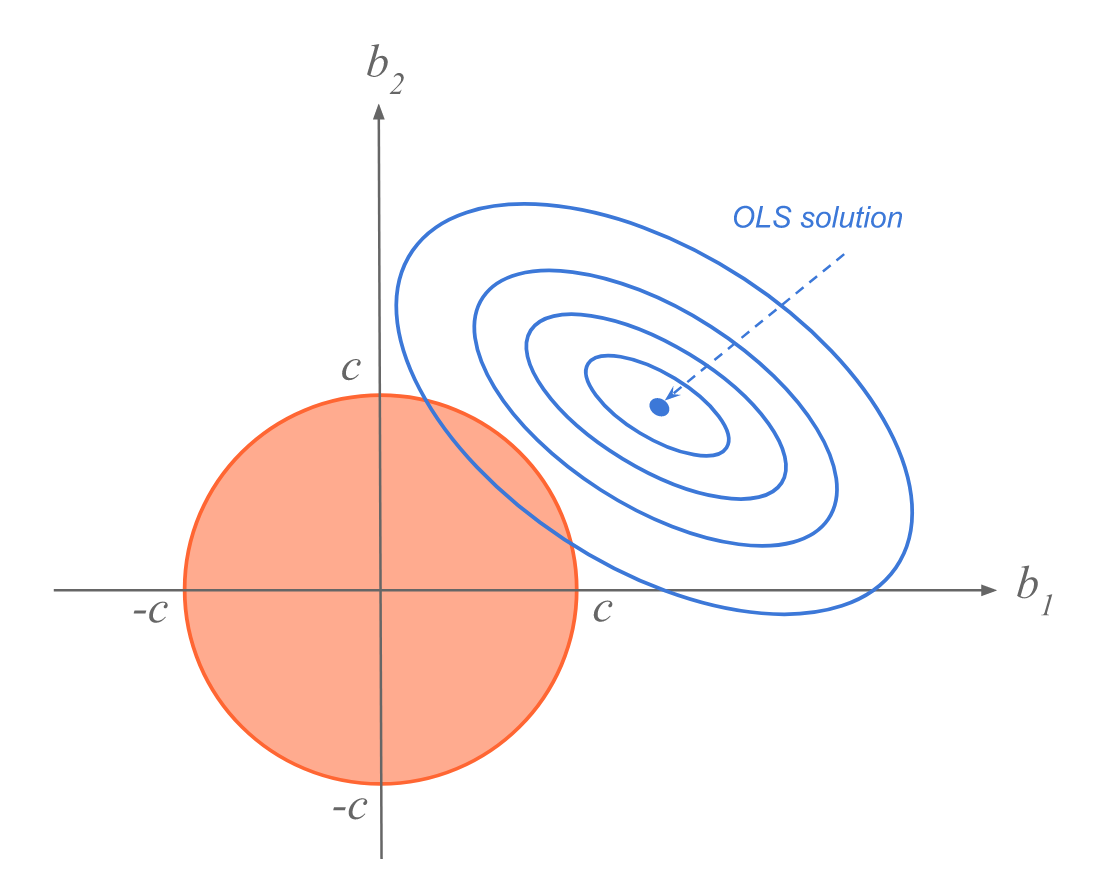
\includegraphics[scale=0.3]{figures/ridge1}
 
\tiny
Fuente: \url{https://allmodelsarewrong.github.io}
\end{figure}


\end{frame}
%----------------------------------------------------------------------%
\begin{frame}[fragile]
\frametitle{Ridge: Intuición en 2 Dimensiones }

\begin{align}
     min_{\beta} E(\beta) &= \sum_{i=1}^n (y_i - x_{i1}\beta_1 - x_{i1}\beta_2)^2  \text{ s.a }   \left( (\beta_1)^2 + (\beta_2)^2 \right) \leq c 
  \end{align}

\begin{figure}[H] \centering
            \captionsetup{justification=centering}
              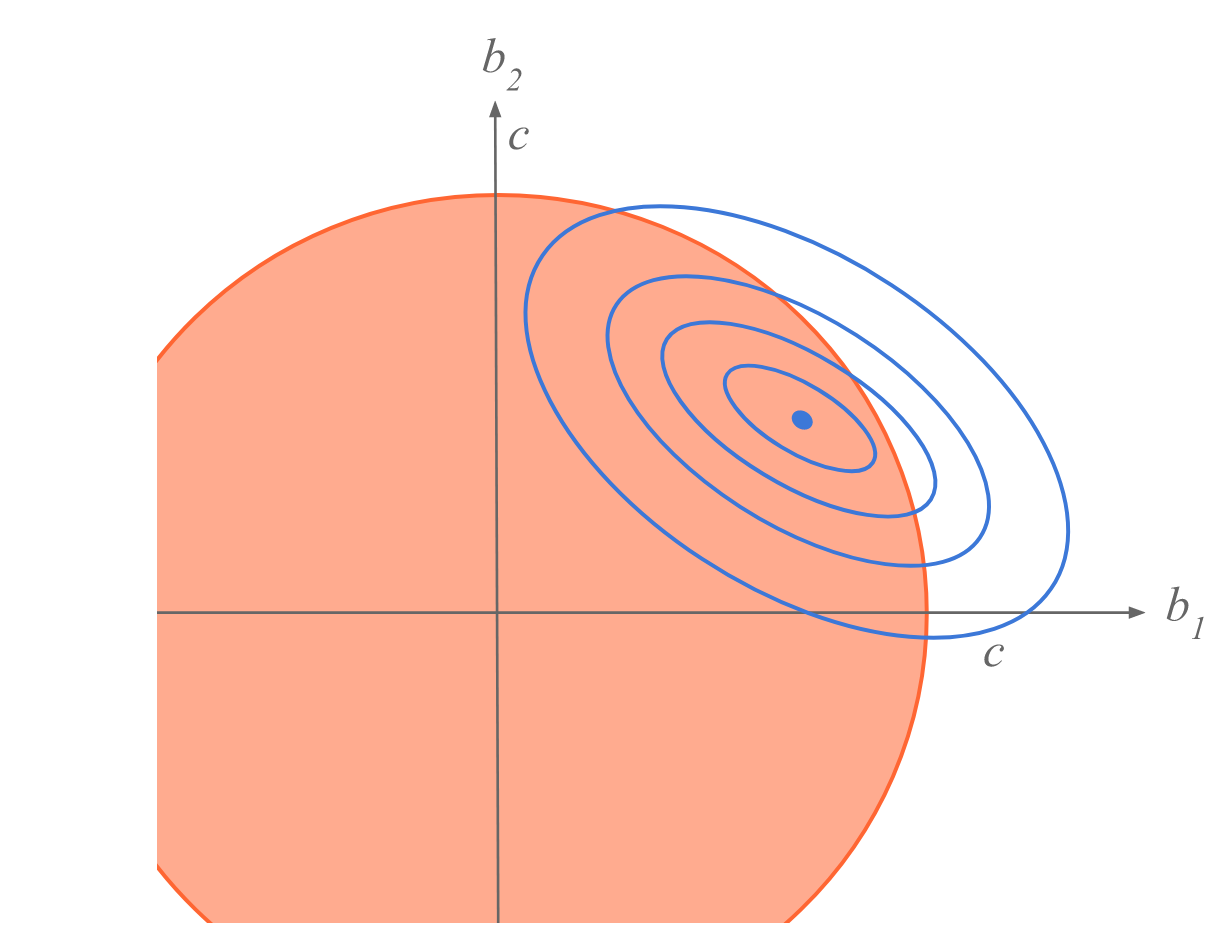
\includegraphics[scale=0.3]{figures/ridge2}
 
\tiny
Fuente: \url{https://allmodelsarewrong.github.io}
\end{figure}


\end{frame}
%----------------------------------------------------------------------%
\begin{frame}[fragile]
\frametitle{Ridge: Intuición en 2 Dimensiones }

\begin{align}
     min_{\beta} E(\beta) &= \sum_{i=1}^n (y_i - x_{i1}\beta_1 - x_{i1}\beta_2)^2  \text{ s.a }   \left( (\beta_1)^2 + (\beta_2)^2 \right) \leq c 
  \end{align}

\begin{figure}[H] \centering
            \captionsetup{justification=centering}
              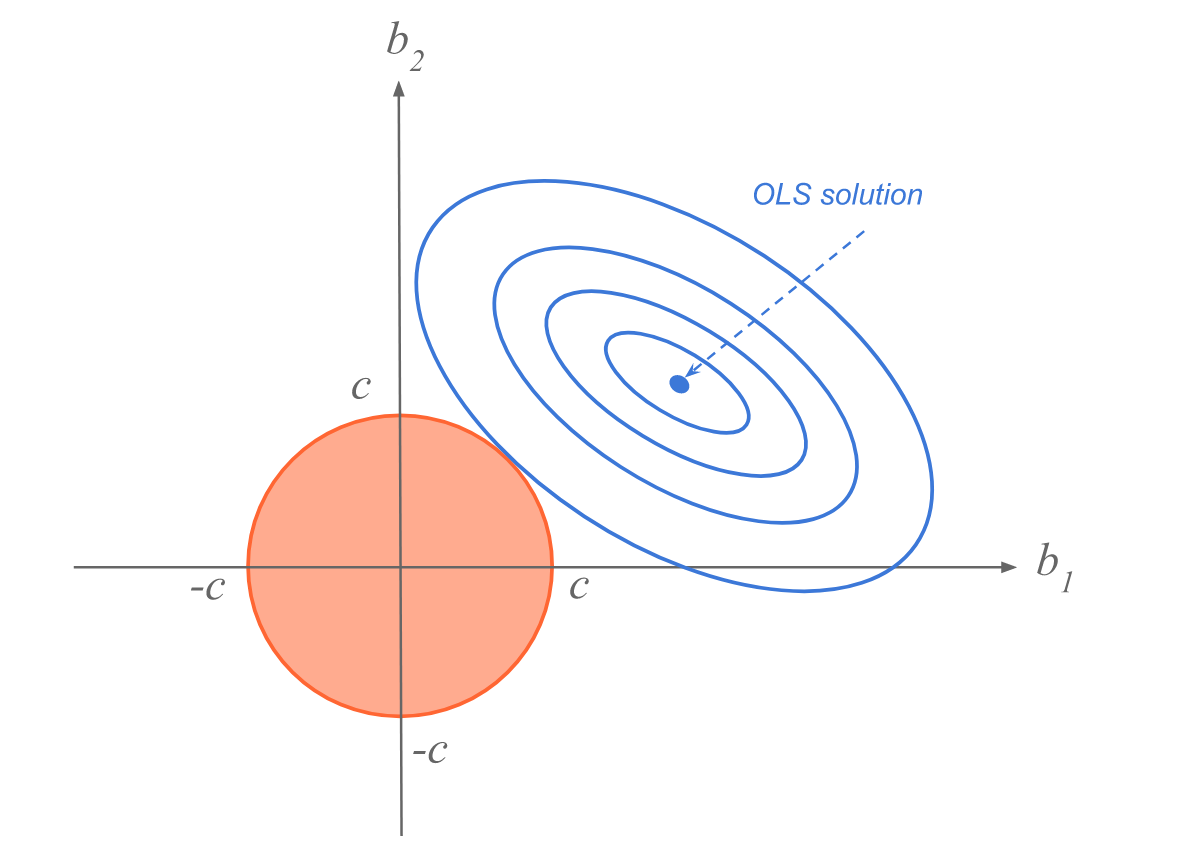
\includegraphics[scale=0.3]{figures/ridge3}
 
\tiny
Fuente: \url{https://allmodelsarewrong.github.io}
\end{figure}


\end{frame}
%----------------------------------------------------------------------%
\begin{frame}[fragile]
\frametitle{Ridge: Intuición en 2 Dimensiones }

\begin{align}
     min_{\beta} E(\beta) &= \sum_{i=1}^n (y_i - x_{i1}\beta_1 - x_{i1}\beta_2)^2  \text{ s.a }   \left( (\beta_1)^2 + (\beta_2)^2 \right) \leq c 
  \end{align}

\begin{figure}[H] \centering
            \captionsetup{justification=centering}
              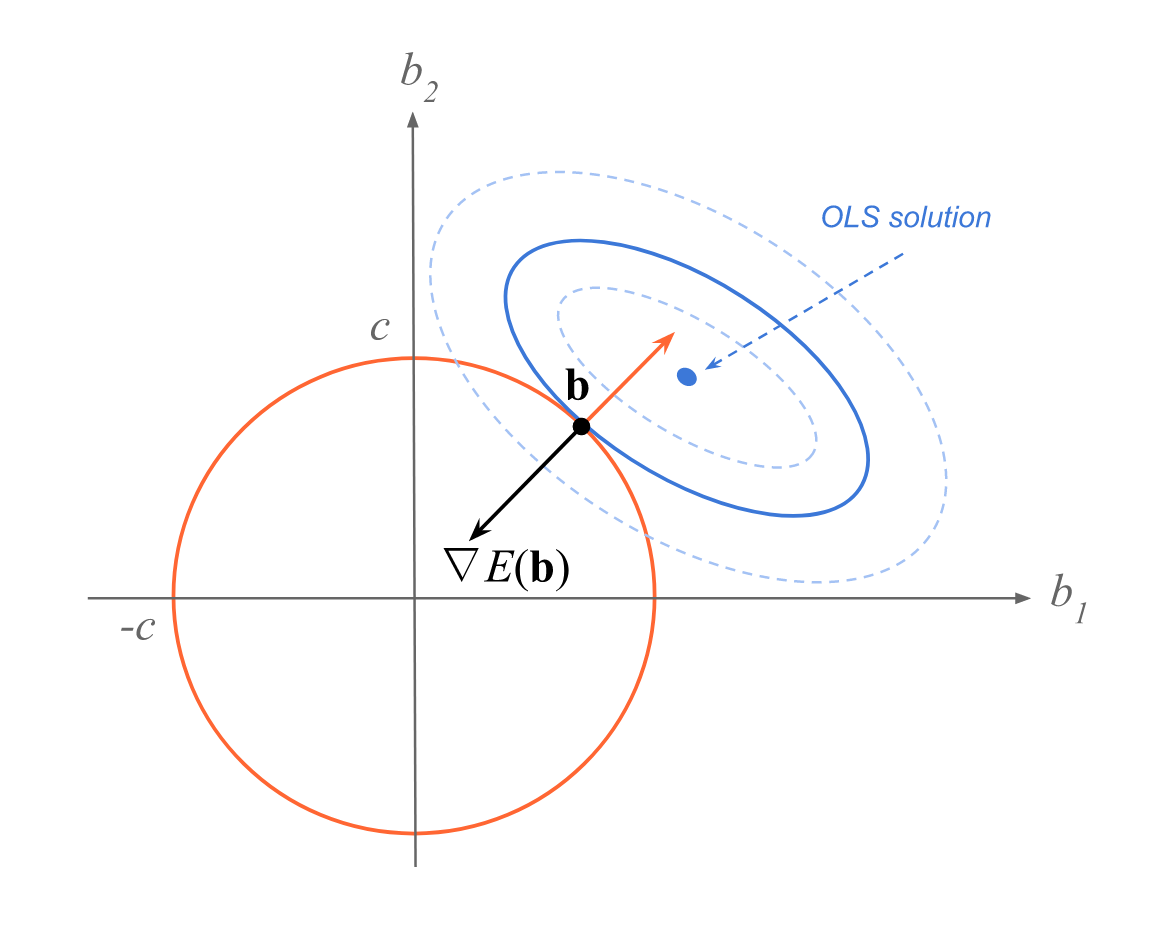
\includegraphics[scale=0.3]{figures/ridge4}
 
\tiny
Fuente: \url{https://allmodelsarewrong.github.io}
\end{figure}

\end{frame}


%----------------------------------------------------------------------%
\begin{frame}[fragile]
\frametitle{Recap}
\begin{itemize}
    \item Asegurar cero sesgo dentro de muestra crea problemas fuera de muestra: trade-off Sesgo-Varianza
    \medskip
    \item Las técnicas de machine learning fueron desarrolladas para hacer este trade-off de forma empírica.
    \medskip
    \begin{align}
min_{\beta} E(\beta) = \sum_{i=1}^n (y_i-\beta_0 - x_{i1}\beta_1 - \dots - x_{ip}\beta_p)^2 + \lambda \sum_{j=1}^p R(\beta_j)
\end{align}
\item $\lambda$ es el precio al que hacemos este trade off
\medskip
\item Próxima clase: como elegimos este $\lambda$
 
\end{itemize}
 

 \end{frame}


%----------------------------------------------------------------------%
\end{document}
